\documentclass[../../D1.tex]{subfiles}

\begin{document}

\subsubsection{Pruning}\label{sec:Pruning}
Network pruning is the process of removing unimportant connections, leaving only the most informative connections.
There has been a substantial amount of research into how pruning can be used to reduce overfitting and network complexity~\autocite{hansonComparingBiasesMinimal,hassibiSecondOrderDerivatives,lecunOptimalBrainDamage,stromPhonemeProbabilityEstimation1997}, but more recent research shows that some pruning methodologies can produce pruned networks with no loss of accuracy~\autocite{hanLearningBothWeights2015}.

\subsubsection{Quantization and Weight Sharing}\label{sec:Quantization}

Quantization is the process of limiting the number of bits used to represent each weight within a network, this process results in many weights using identical or very close weight values. 
These repeated weight values creates an ideal situation to use weight sharing techniques.

The paper Deep Compression by Han et al~\autocite{hanDeepCompressionCompressing2016} weight sharing is taken a step further and clustering is employed to gather the quantized weights into bins (whose value is denoted by the centroid of that bin) then an index is assigned to each weight that points to the weights corresponding bin, the bins value is the centroid of that cluster, which is further fine-tuned by subtracting the sum of the gradients for each weight in the bin their respective centroid see Fig.~\ref{fig:QuantizationClust}.  

\begin{figure}[H]
    \begin{center}
        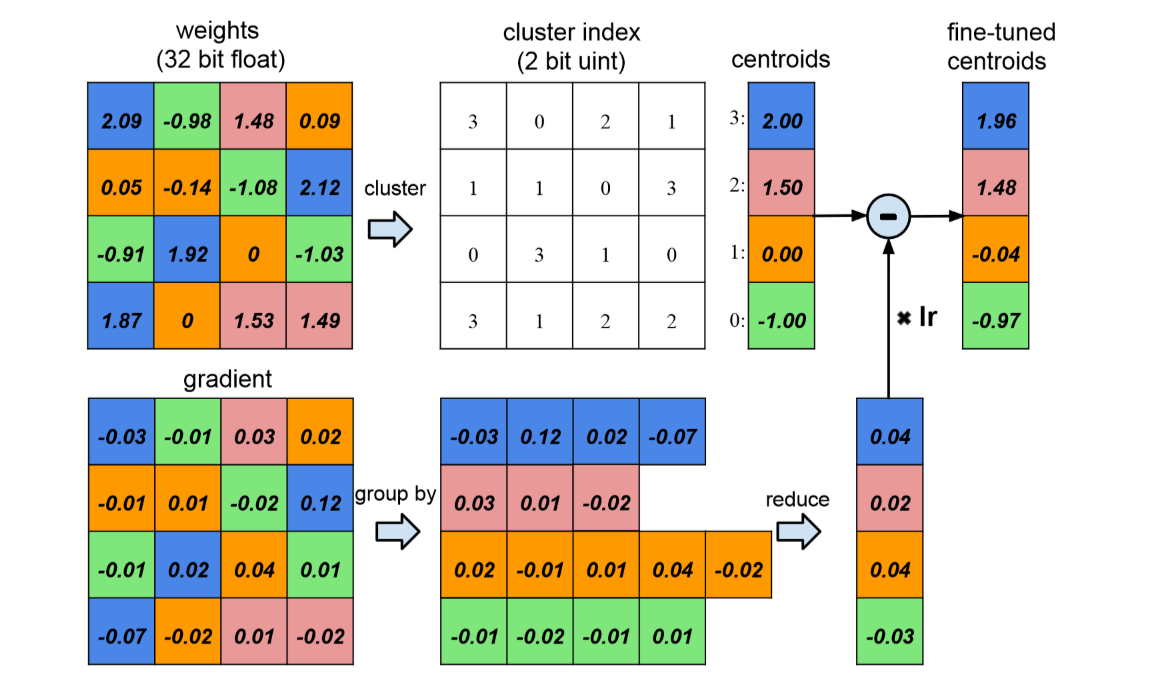
\includegraphics[width=1\textwidth]{quantization_clustering.png} 
    \end{center}
    
    \caption{Weight sharing by quantization with centroid fine-tuning using gradients\\ \textbf{(Adopted figure from~\autocite{hanDeepCompressionCompressing2016})}}
    \label{fig:QuantizationClust}   
\end{figure}

\subsubsection{Distillation}\label{sec:Distillation}

\subsubsection{Low-rank Factorization}\label{sec:lrFactorization}

\subsubsection{Network Design Strategies}\label{sec:NetworkDesignStrat}

\end{document}
